\chapter{Intelligent AI Agents}

\section{Intelligent Agent}

An intelligent agent is an autonomous entity which act upon an
environment using sensors and actuators for achieving goals.

\begin{minipage}{0.6\textwidth}
\begin{itemize}[parsep=0.5em]
    \item An AI agent must have the ability to \textbf{perceive} the environment.
    \item The observation must be used to \textbf{make decisions}.
    \item Decision should result in an \textbf{action}.
    \item The action taken by an AI agent must be a \textbf{rational action}.
\end{itemize}
\end{minipage}%
\hfill
\begin{minipage}{0.4\textwidth}
   \centering
   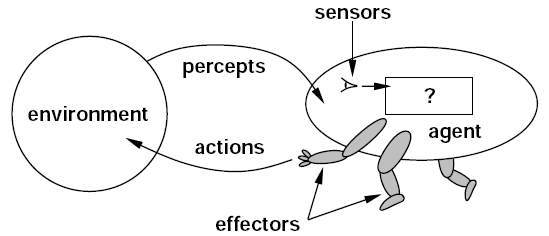
\includegraphics[width=\textwidth]{figures/AI Agent Environment.png}
   \label{fig:ai-agent-environment}
\end{minipage}%

\subsection{Rational Agent}

A rational agent is an agent which has clear preference, models uncertainty, and acts in a way to maximize its performance measure with all possible actions.

The rationality of an agent is measured by its performance measure.
\begin{itemize}[parsep=0.5em]
   \item Performance measure which defines the \textbf{success criterion}.
   \item Agent \textbf{prior knowledge} of its environment.
   \item \textbf{Best possible actions} that an agent can perform.
   \item The \textbf{sequence of percepts}.
\end{itemize}

\section{Agent Environment in AI}

The environment is everything surrounding an agent (but not part of it), where the agent lives, operates and provides the agent with something to sense and act upon it.

\subsection*{Features of Environment}

\begin{itemize}
   \item 
   \textbf{Fully observable}: If the agent's sensors can access the complete state at each moment.\\
	\textbf{Partially observable}: If the agent can only sense part of the state.\\
	\textbf{Unobservable}: If the agent has no sensors to perceive the environment.

   \item 
   \textbf{Deterministic Environment:} If an agent's current state and selected action can completely determine the next state of the environment.\\ 
   \textbf{Stochastic Environment:} If the next state is random and cannot be fully predicted by the agent.


   \item
   \textbf{Competitive Environment:} If an agent competes against another agent to optimize the outcome.\\
   \textbf{Collaborative Environment:} If multiple agents cooperate to achieve a desired outcome.
   
   
   \item
   \textbf{Single-Agent Environment:} Consists of only one agent.\\
   \textbf{Multi-Agent Environment:} Involves more than one agent.
   
   
   \item
   \textbf{Dynamic Environment:} Constantly changes in response to an agent's actions.\\
   \textbf{Static Environment:} An idle environment with no change in its state.
   
   
   \item
   \textbf{Discrete}: An environment with a finite number of actions is called a discrete environment\\
   \textbf{Continuous}: An environment where actions cannot be numbered is called a continuous environment.
   
   
   \item
   \textbf{Episodic environment}: Agent's actions are divided into independent episodes. In each episode, the agent receives input from the environment and performs the corresponding action.\\
   \textbf{Sequential environment}: Agent's next action depends on past and planned actions that is previous decisions affect future ones.
   
   
   \item
   \textbf{Known Environment:} The agent knows the results of all actions and can make decisions based on complete information, though it may still be partially observable.\\
   \textbf{Unknown Environment:} The agent must learn how the environment works to perform actions. It may be fully observable but requires gaining knowledge to decide.
\end{itemize}


\section{PEAS}

\begin{tabularx}{\textwidth}
{|>{\centering\arraybackslash}p{2cm}|C|C|C|C|}\hline
   \textbf{Name} & \textbf{Performance measure} & \textbf{Environment} & \textbf{Actuators} & \textbf{Sensors} \\\hline
   
   Automated taxi driver 
   & Safe, fast, legal, comfortable trip, maximize profits 
   & Roads, other traffic, pedestrians, customers 
   & Steering wheel, accelerator, brake, signal, horn 
   & Cameras, sonar, speedometer, GPS, odometer, engine sensors, keyboard \\\hline

   Dengue diagnosis system
   & Healthy patient, minimize cost, maximize efficiency, minimize False positive and False Negative
   & Patient, hospital, staff
   & Screen display (questions, tests, diagnoses, treatments, referrals)
   & Temperature Sensor, Keyboard (entry of symptoms, findings, patient's answers)
   \\\hline

   Trash picking robot
   & Cleanliness, amount of trash collected, efficiency, minimal damage, safety
   & University campus, CSE void space, obstacles, trash bins, people
   & Motors \& wheels, robotic arm/gripper, trash bin compartment
   & Camera, proximity sensors, touch sensors, weight sensor, GPS
   \\\hline

   Strawberry classification agent
   & Accurate classification of ripe/unripe/bad, speed, minimal misclassification, maximize throughput
   & Strawberry processing plant, conveyor belt, strawberries, and foreign materials
   & Conveyor belt control, sorting arms, reject bin actuator
   & Camera (visual sensor), color/shape sensor, weight sensor, IR sensor
   \\\hline

   UAP Environment Monitoring Agent
   & Accurate detection/report illegal activities, timely alerts, minimal false alarms, continuous coverage, efficiency
   & UAP campus, buildings, outdoor areas, people, vehicles, events, weather conditions
   & Drone motors/propellers, camera gimbal, alarm/notification system, lights, speakers
   & Cameras (visual sensors), microphones, GPS, motion sensors, environmental sensors, Wi-Fi module
   \\\hline

   AlphaGo
   & Win the game, maximize score, minimize mistakes, play efficiently, follow rules
   & Go board, opponent (human player), game rules, time constraints
   & Move generator (places stones on board), resign action
   & Camera for board state input, opponent's moves, game clock
   \\\hline
\end{tabularx}